\documentclass[10pt]{scrartcl}

\usepackage[utf8]{inputenc}
\usepackage{tabularx}
\usepackage[ngerman]{babel}
\usepackage[automark]{scrpage2}
\usepackage{amsmath,amssymb,amstext}
%\usepackage{mathtools}
\usepackage[]{color}
\usepackage[]{enumerate}
\usepackage{graphicx}
\usepackage{lastpage}
\usepackage[perpage,para,symbol*]{footmisc}
\usepackage{listings} 
\usepackage[pdfborder={0 0 0},colorlinks=false]{hyperref}
\usepackage[numbers,square]{natbib}
\usepackage{color}
\usepackage{colortbl}
\usepackage{listings}
\usepackage{a4wide}
\usepackage{xspace}
\usepackage{listings}
\usepackage{hyperref}
\usepackage{epstopdf}

\lstset{numbers=left, numberstyle=\tiny, numbersep=5pt, breaklines=true, showstringspaces=false} 

%changehere
\def\titletext{TH1 Praktikum 1 : Ausarbeitung}
\def\titletextshort{Praktikum 1}
\author{Carsten Noetzel, Armin Steudte}

\title{\titletext}

%changehere Datum der Übung
\date{23.03.2012}

\pagestyle{scrheadings}
%changehere
\ihead{TH1, Padberg}
\ifoot{Generiert am:\\ \today}

\cfoot{Carsten Noetzel, Armin Steudte}


\ohead[]{\titletextshort}
\ofoot[]{{\thepage} / \pageref{LastPage}}

\setlength{\parindent}{0.0in}
\setlength{\parskip}{0.1in}

\begin{document}
\maketitle

\setcounter{tocdepth}{3}
\tableofcontents
\listoffigures
%\lstlistoflistings

\section{Aufgabe 1 - Aufbau des Petrinetzes}

\begin{figure}[htbp]
	\centering	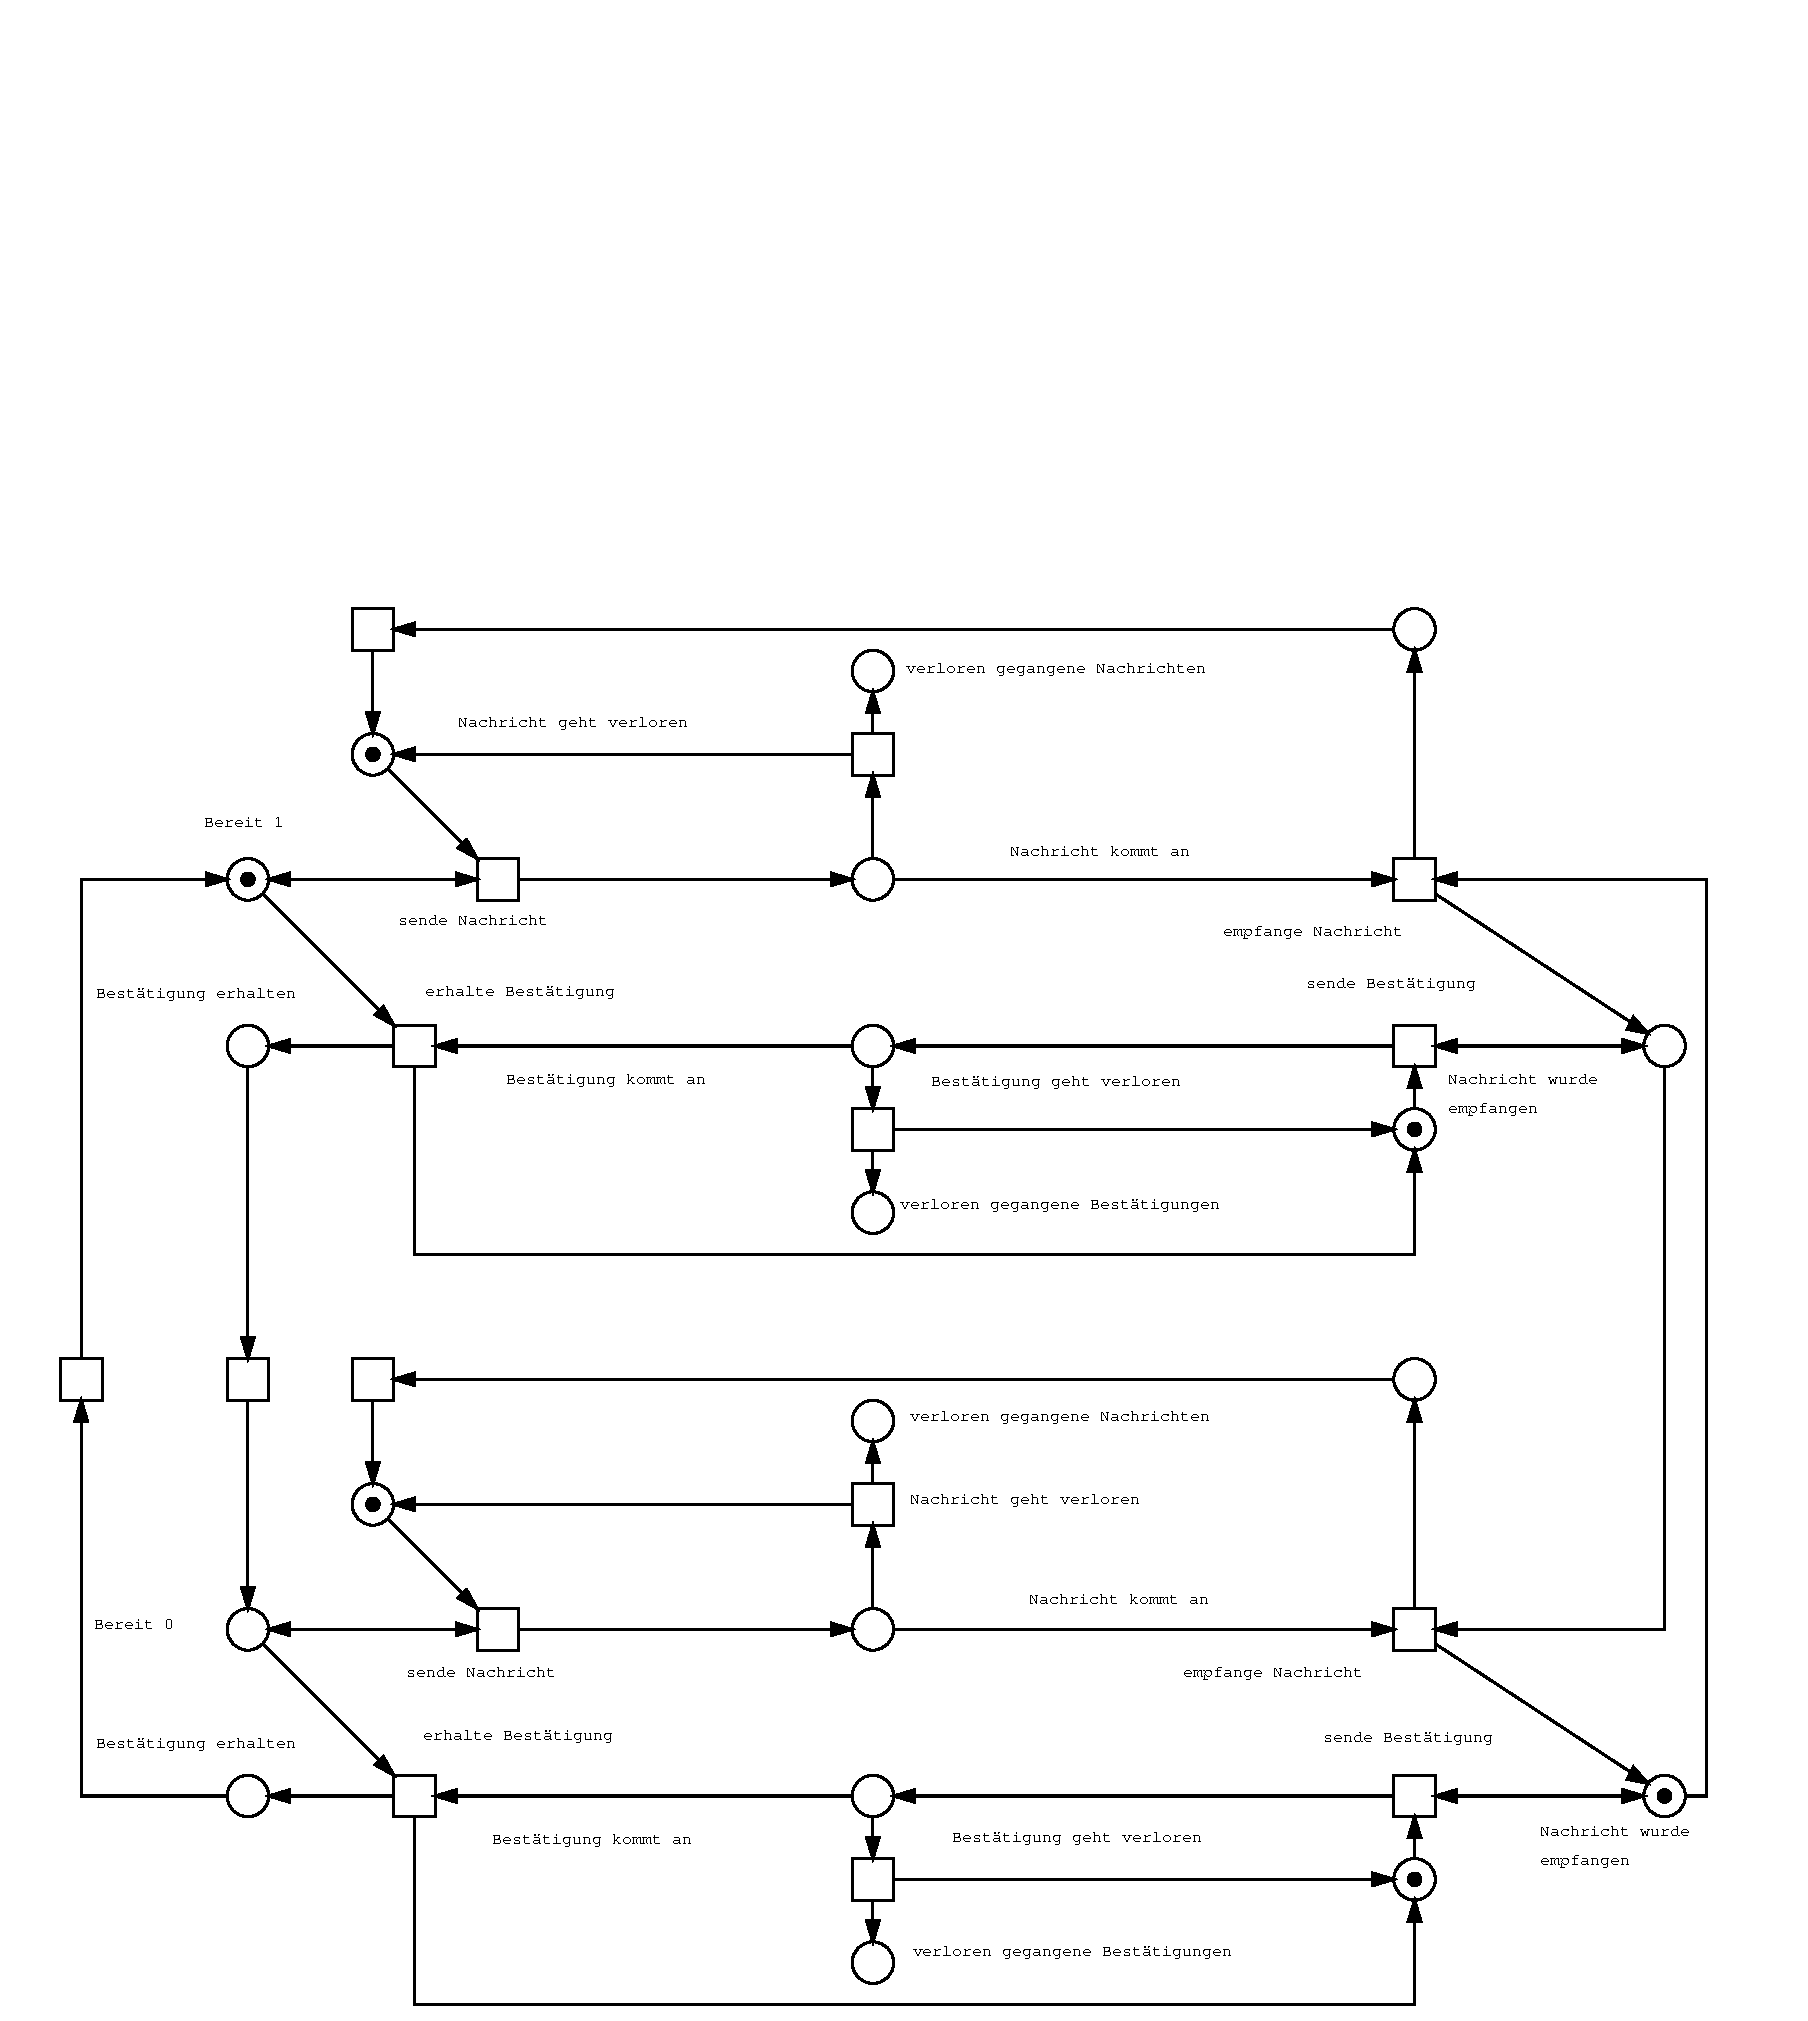
\includegraphics[width=1.0\textwidth]{Grafiken/Praktikum1_1.eps}
	\caption{Petrinetz}
	\label{fig:Netz}
\end{figure} 

\section{Aufgabe 2 - Erläuterungen zur Modellierung}

\section{Aufgabe 3 - Begründung der Korrektheit}

\section{Aufgabe 4 - Nachrichtenverlust}

\section{Aufgabe 5 \& 6 - Erweiterung des Systems}
\subsection{Von 20 Nachrichten maximal 1 Nachricht Verlust}
\subsection{Pro gesendeter Nachricht maximal 20 Nachrichten Verlust}



\end{document}

